\documentclass[fleqn, a4paper, 11pt, russian]{article}

\usepackage[utf8]{inputenc}
\usepackage[T1, T2A]{fontenc}
\usepackage[english, main = russian]{babel}
\usepackage{indentfirst}
\parindent 1.27cm
\usepackage{graphicx}
\usepackage{natbib}
\usepackage{caption, subcaption}
\usepackage[top=2cm, left=2cm, right=2cm, left=2cm]{geometry}
\usepackage{amsmath} %Для работы с матрицами
\usepackage{amssymb}
\usepackage{ragged2e}
\usepackage{makecell}

\usepackage{listings}
\usepackage{inconsolata}

\lstset{
	basicstyle = \ttfamily,
}


\graphicspath{{Images/}}

\newcolumntype{L}[1]{>{\raggedright\let\newline\\\arraybackslash\hspace{0pt}}m{#1}}
\newcolumntype{C}[1]{>{\centering\let\newline\\\arraybackslash\hspace{0pt}}m{#1}}
\newcolumntype{R}[1]{>{\raggedleft\let\newline\\\arraybackslash\hspace{0pt}}m{#1}}

\newcommand{\R}{\mathbb{R}}

\captionsetup[figure]{name = Рисунок, labelsep = endash}
\captionsetup[table]{name = Таблица, labelsep = endash, justification=raggedright, singlelinecheck=false}
\setlength{\mathindent}{0pt}

\begin{document}
	\newcommand\tline[2]{$\underset{\text{#1}}{\text{\underline{\hspace{#2}}}}$}
\newcommand\nameLine[3]{$\underset{\text{#1}}{\text{\underline{\text{#2}\hspace{#3}}}}$}

\begin{titlepage}
	\centering
	{\fontsize{12pt}{5cm}\selectfont \bfseries Министерство образования и науки Российской Федерации} \\ \vspace{0.5cm}
	{\fontsize{7pt}{5cm}\selectfont ФЕДЕРАЛЬНОЕ ГОСУДАРСТВЕННОЕ АВТОНОМНОЕ ОБРАЗОВАТЕЛЬНОЕ УЧРЕЖДЕНИЕ ВЫСШЕГО ПРОФЕССИОНАЛЬНОГО ОБРАЗОВАНИЯ} \\ 
	\vspace{1cm}
	{\fontsize{12pt}{5cm}\selectfont \bfseries САНКТ-ПЕТЕРБУРГСКИЙ УНИВЕРСИТЕТ ИНФОРМАЦИОННЫХ ТЕХНОЛОГИЙ, МЕХАНИКИ И ОПТИКИ} \\ \vspace{1.5cm}

	{\fontsize{14pt}{5cm}\selectfont Кафедра \hspace{1cm} \underline{Систем Управления и Информатики}  \hspace{1cm} Группа \underline{Р3340}} \\ 
	\vspace{2cm}

	{\fontsize{20pt}{5cm}\selectfont \bfseries Расчётная работа} \\ %%
	{\fontsize{20pt}{5cm}\selectfont \bfseries “Решение задачи построения ПИ-регулятора”} \\ %%
	{\fontsize{16pt}{5cm}\selectfont по курсу “Специальные разделы теории управления”} \\
	\vspace{1.5cm}

	\flushleft

	{Выполнил \hspace{2cm} \nameLine{(фамилия. и.о.)}{Алякин С.П.}{6.5cm} (подпись)} \\
	\vspace{2cm}

	{Проверил \hspace{2cm} \nameLine{(фамилия, и.о.)}{}{9cm} (подпись)}\\
	\vspace{5cm}

	"\underline{\hspace{0.7cm}}"\hspace{0.2cm}\underline{\hspace{2cm}}\hspace{0.2cm}20\underline{ 17 }г. \hspace{2cm} Санкт-Петербург, \hspace{2cm} 20\underline{ 17 }г. \\ \vspace{1cm}

	Работа выполнена с оценкой \hspace{1cm} \underline{\hspace{8cm}} \\ 
	\vspace{1cm}
	Дата защиты "\underline{\hspace{0.7cm}}"\hspace{0.2cm}\underline{\hspace{2cm}}\hspace{0.2cm}20\underline{ 17 }г.
		
\end{titlepage}
	
	\section*{Цель работы}
	Для заданного объекта управления спроектировать пропорционально-интегральный регулятор, обеспечивающий в замкнутой системе требуемое время переходного процесса и значение перерегулирования.
	\section*{Исходные данные}
	Задан объект управления, структурная схема которого представлена на рисунке \ref{struct}.
	\begin{figure}[ht!]
		\centering
		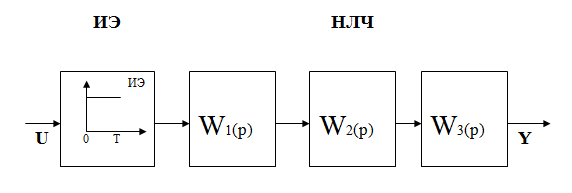
\includegraphics[scale = 1]{struct}
		\caption{Общая структура объекта управления}
		\label{struct}
	\end{figure}
	
	Для проектирования были выданные исходные данные, представленные в таблице.
	\begin{table}[h]
		\caption{Исходные данные}
		\begin{tabular}{| c | c | c | c | c | c | c | C{2cm} | C{2cm} | C{2cm}|}
			\hline
			T & \multicolumn{2}{c|}{$W_1$} & \multicolumn{2}{c|}{$W_2$} & \multicolumn{2}{c|}{$W_3$} & Тип регулятора & Время переходного процесса & Перерегулирование\\
			\hline
			& $K_1$ & $T_1$ &$K_2$ & $T_2$ & $K_3$ & $T_3$ & & &\\
			\hline
			[c] & --- & [c] & --- & [c] & --- & [c] & & [c] & [\%]\\
			\hline
			0,0040 & --- & --- & 500,00 & 0,10 & 0,25 & Интегратор & ПИ & 0,150 & 30,00\\
			\hline
		\end{tabular}
	\end{table}
	\clearpage
	\section{Составление уравнения Вход-Состояние-Выход в дискретной форме для объекта управления}
	Опишем передаточную функцию $\displaystyle{\frac{500}{0,1s + 1}}$ в виде интегратора и коэффициентов обратной связи:
	\begin{align}
		&&\dot{x_2} = -k_3k_4x_2 + k_4u\\
		&&sx_2 + k_3k_4x_2 = k_4u\\
		&&x_2 = \frac{\displaystyle{\frac{1}{k_3}}u}{\displaystyle{\frac{1}{k_3k_4}}s + 1}
	\end{align}
	
	Из полученного выражения найдём коэффициенты $k_3 = 0,002, k_4 = 5000$	
	
	Опишем систему уравнениями Вход-Состояние-Выход:
	\begin{align} \label{dsym}
		&&\begin{cases}
			\dot{x} = A_\text{н}x + И_\text{н}U\\
			Y = CX
		\end{cases} , \text{где } A_\text{н} = \begin{bmatrix}
			0 & k_2\\
			0 & -\displaystyle{\frac{1}{T_2}}
		\end{bmatrix}, B_\text{н} = \begin{bmatrix}
			0\\
			\displaystyle{\frac{k_1}{T_1}}
		\end{bmatrix}, C = \begin{bmatrix}
			1 & 0
		\end{bmatrix}
	\end{align}
	где $x(k)\in\R^2$ --- вектор состояния дискретной системы, $u(k)\in\R^1$ --- управляющее воздействие, $y(k)\in\R^2$ --- регулируемая переменная, $A_\text{н}$ -- $(2\times 2)$ --- дискретизированная матрица состояния, определяющая динамические свойства системы, $B_\text{н}$ -- $(2 \times 1)$ --- дискретизированная матрица выходов, определяющая точки приложения к ОУ управляющих воздействий, $C$ -- $(1 \times 2)$ --- матрица выходов, определяющая связь между переменными состояния и выходными переменными.
	
	Подставив в (\ref{dsym}) известные значения параметров $k_1 = 500, k_2 = 0,25, T_1 = 0,1$, получим следующие матрицы:
	\begin{align}
		&&A_\text{н} = \begin{bmatrix}
			0 & 0,25\\
			0 & -10
		\end{bmatrix}, B_\text{н} = \begin{bmatrix}
			0\\
			5000
		\end{bmatrix}, C = \begin{bmatrix}
			1 & 0
		\end{bmatrix}
	\end{align}
	
	Для перехода от непрерывной модели к дискретной воспользуемся соотношениями
	\begin{align} \label{c2d}
		&A_d = \sum_{i = 0}^{\infty}\displaystyle{\frac{A^iT^i}{i!}}; &&B_d = \sum_{i = 1}^{\infty} \displaystyle{\frac{A^{i-1}T^i}{i!}}B; &C_d = C
	\end{align}
	
	Чтобы рассчитать дискретизированные матрицы, напишем программу в среде matlab, листинг которой приведён в приложении А. В результате работы программы были получены следующие результаты:
	\begin{align}
		\label{dmtrxA}
		&&A_d = \begin{bmatrix}
			1 & 0,0009802640211919198\\
			0 & 0,960789439152323
		\end{bmatrix},\\
		\label{dmtrxB}
		&&B_d = \begin{bmatrix}
			0,009867989404040\\
			19,605280423838394
		\end{bmatrix},\\
		\label{dmtrxC}
		&&C_d = \begin{bmatrix}
			1 & 0
		\end{bmatrix}.
	\end{align}
	
	Теперь получим систему уравнений Вход-Состояние-Выход в дискретной форме, подставив матрицы (\ref{dmtrxA}), (\ref{dmtrxB}) и (\ref{dmtrxC}) в уравнение (\ref{dsym}):
	\begin{align}
		&&\begin{cases}
			\begin{bmatrix}
				x_1(k+1)\\
				x_2(k+1)
			\end{bmatrix} = \begin{bmatrix}
				1 & 0,0009802640211919198\\
				0 & 0,960789439152323
			\end{bmatrix} \cdot \begin{bmatrix}
				x_1(k)\\
				x_2(k)
			\end{bmatrix} + \begin{bmatrix}
				0,009867989404040\\
				19.605280423838394
			\end{bmatrix} \cdot u(k)\\			
			y(k) = \begin{bmatrix}
				1 & 0
			\end{bmatrix} \cdot \begin{bmatrix}
				x_1(k)\\
				x_2(k)
			\end{bmatrix}
		\end{cases}
	\end{align}
	\clearpage
	\section{Переход к передаточной функции объекта управления}
	Для перехода от уравнений Вход-Состояние-Выход к передаточной функции объекта необходимо воспользоваться следующим соотношением:
	\begin{align}
		&&W(z) = C_d(zI - A_d)^{-1}B_d
	\end{align}
	
	Решив данное уравнение при помощи среды Matlab, получим функцию:
	\begin{align}
		&&W(z) = \displaystyle{\frac{0,009867989404040z + 0,009737291019798}{z^2 - 1,960789439152323z + 0,960789439152323}}
	\end{align}
	
	Найдём корни характеристического уравнения
	\begin{align}
		\lambda^2 - 1,9608\lambda + 0,9608 = 0\\
		&\lambda_1 = 1;  &\lambda_2 = 0,9608
	\end{align}
	
	Получим переходные характеристики полученной дискредитированной передаточной функции и исходной непрерывной передаточной функции, воспользовавшись функцией Matlab --- stepplot. Полученный в ходе работы функции график представлен на рисунке \ref{hWz}.
	\begin{figure}[ht!]
		\centering
		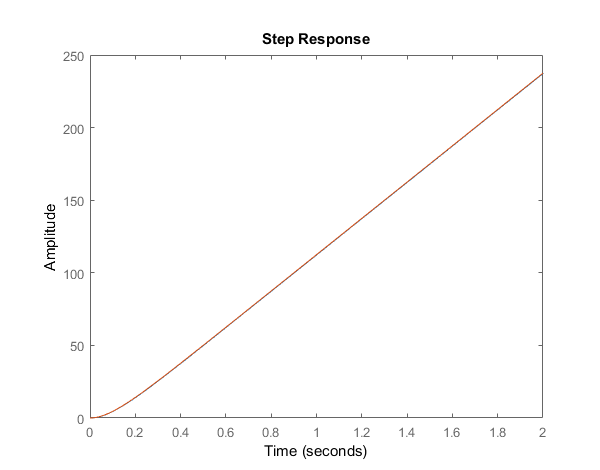
\includegraphics[width = 0.8\textwidth]{stepresp}
		\caption{Переходная характеристика}
		\label{hWz}	
	\end{figure}
	
	Как видно на представленном графике, переходные процессы совпадают, следовательно расчёт был проведён правильно.
	\clearpage
	\section{Расчёт регулятора и его математическая модель}
	Сведём задачу к выбору матриц эталонной модели $\Gamma, H$ и решению уравнения типа Сильвестра:
	\begin{align} \label{sylv}
		&&\begin{cases}
			\overline{M}\Gamma - \overline{A}\overline{M} = -\overline{B}H\\
			\overline{K} = H\overline{M^{-1}}
		\end{cases}
	\end{align}
	\subsection{Проверка дискретного ОУ на управляемость}
	Найдём матрицу управляемости
	\begin{align}
		&&U_d = \begin{bmatrix}
			B_d & A_dB_d
		\end{bmatrix}
	\end{align}
	воспользовавшись функцией ctrb Matlab. Полученная матрица
	\begin{align}
		&&U_d = \begin{bmatrix}
			0,009867989404040 & 0,029086340428907\\
			19,605280423838394 & 18,836546382843710
		\end{bmatrix}.
	\end{align}
	Проверим матрицу на управляемость
	\begin{align} \label{Uctrl}
		&rank(U_d) = 2 = n, &&det(U_d) = -0,384367020497341 \neq 0.
	\end{align}
	
	Из (\ref{Uctrl}) видно, что пара матриц $A_d, B_d$ полностью управляема.
	
	\subsection{Формирование эталонной модели}
	Исходя из условия о том, что значение перерегулирования не должно превышать 30\% и того, что наша система имеет второй порядок, выберем полином Ньютона 3 порядка порядка в качестве требуемого характеристического полинома, имеющего вид
	\begin{align} \label{Btrw}
		&&\lambda^3 + 3\omega_0\lambda^2 + \omega_0^2\lambda + \omega_0^3
	\end{align}
	
	Чтобы найти требуемое значение $\omega_0$ построим переходную характеристику звена с передаточной характеристикой
	\begin{align}
		&&W(s) = \displaystyle{\frac{1}{s^3 + 3s^2 + 3s + 1}}
	\end{align}
	при единичном входном воздействии. В ходе моделирования был получен график, представленный на рисунке \ref{hWw}.
	\begin{figure}[ht!]
		\centering
		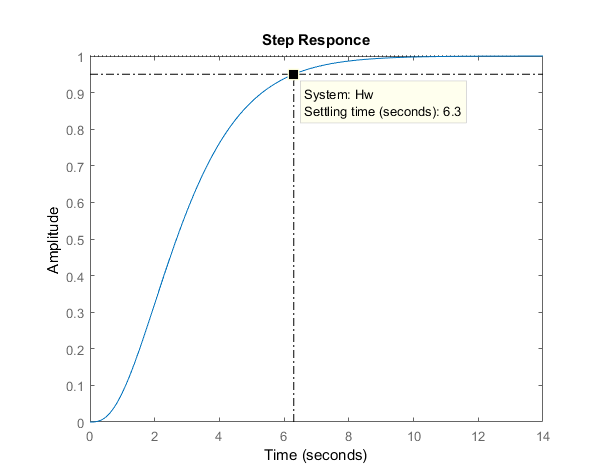
\includegraphics[scale=0.75]{hWw}
		\caption{График нормированной переходной функции}
		\label{hWw}
	\end{figure}
	Из него, учтя, что $\Delta = 0,05$, найдём значение переходного процесса $t_\text{п}^* = 6,3 c$. Рассчитаем $\omega_0$ по следующей формуле
	\begin{align}
		&&\omega_0 = \frac{t_\text{п}^*}{t_\text{п}} = \frac{6,3}{0,15} = 42,
	\end{align}
	где $t_\text{п}$ --- требуемое время переходного процесса. Подставим полученное значение $\omega_0$ в выражение (\ref{Btrw}).
	\begin{align}
		&&\lambda^3 + 126\lambda^2 + 5292\lambda + 74088
	\end{align}

	Найдём корни полученной непрерывной эталонной модели
	\begin{align}
		&&\lambda_{1, 2, 3}= -42
	\end{align}
	
	Так как мы имеем 3 одинаковых корня вида $\lambda_{1, 2, 3}$, то матрицы $\Gamma_d$ и $H,$ построенная из условия наблюдаемости пары $\Gamma_d, H$, будут иметь вид
	\begin{align}
		&&\Gamma = \begin{bmatrix}
			\lambda & 1 & 0\\
			0 & \lambda & 1\\
			0 & 0 & \lambda
		\end{bmatrix} = \begin{bmatrix}
			-42 & 1 & 0\\
			0 & -42 & 1\\
			0 & 0 & -42
		\end{bmatrix},
	\end{align}
	\begin{align}
		&&H = \begin{bmatrix}
			1 & 0 & 0
		\end{bmatrix}
	\end{align}
	
	Получим матрицу $\Gamma$ в дискретном пространстве при помощи функции Matlab\\ \texttt{Gd = expm(G*0.004)}:
	\begin{align}
		&&\Gamma_d = \begin{bmatrix}
			0,845353834684659 & 0,003381415338739 & 0,000006762830677477263\\
			0 & 0,845353834684659 & 0,003381415338739\\
			0 & 0 & 0,845353834684659
		\end{bmatrix}
	\end{align}
	
	\subsection{Нахождение матриц расширенной модели ВСВ}
	Найдём матрицы:
	\begin{align}
		&&\overline{A_\text{н}} = \begin{bmatrix}
			0 & C\\
			0 & A_\text{н}
		\end{bmatrix} = \begin{bmatrix}
			0 & 1 & 0\\
			0 & 0 & 0,25\\
			0 & 0 & -10
		\end{bmatrix}\\
		&&\overline{B_\text{н}} = \begin{bmatrix}
			0\\
			B_\text{н}
		\end{bmatrix} = \begin{bmatrix}
			0\\
			0\\
			5000
		\end{bmatrix}
	\end{align}
	
	Найдём значения этих матриц в дискретном пространстве, воспользовавшись формулами (\ref{c2d}):
	\begin{align}
		&&\overline{A_d} = \begin{bmatrix}
			1 & 0,004 & 0,000001973597880808024\\
			0 & 1 & 0,0009802640211919198\\
			0 & 0 & 0,960789439152323
		\end{bmatrix}\\
		&&\overline{B_d} = \begin{bmatrix}
			0,00001320105959598820\\
			0,009867989404040\\
			19,605280423838394
		\end{bmatrix}
	\end{align}
	
	\subsection{Решение уравнения типа Сильвестра}
	Подставив полученные матрицы в первое уравнение системы (\ref{sylv}) рассчитаем матрицу $\overline{M}$, воспользовавшись функцией \texttt{lyap} среды Matlab:
	\begin{align}
		&&\overline{M} = \begin{bmatrix}
		-0,008339994934144 & -0,0004730368613052505	& -0,00001792655436682541\\
		0,472627512917950 & 0,018467003996024 & 0,0005428609746627452\\
		-107,1352046282408 & -2,295590414147008 & -0,049187709752454
		\end{bmatrix}
	\end{align}
	
	Из второго уравнения системы (\ref{sylv}) получим расширенную матрицу линейных стационарных обратных связей:
	\begin{align}
		&&\overline{K} = \begin{bmatrix}
			145,5960607704002 & 7,707573360000006 & 0,032002
		\end{bmatrix},
	\end{align}
	где
	\begin{align}
		&&K_I = 145,5960607704002\\
		&&K_1 = 7,707573360000006\\
		&&K_2 = 0,032002
	\end{align}
	\clearpage
	\section{Результаты синтеза регулятора}
	Схема моделирования рассчитанного апериодического регулятора приведена на рисунке \ref{finModel}. Результат реакции системы представлен на рисунке \ref{fin}.
	\begin{figure}[ht!]
		\centering
		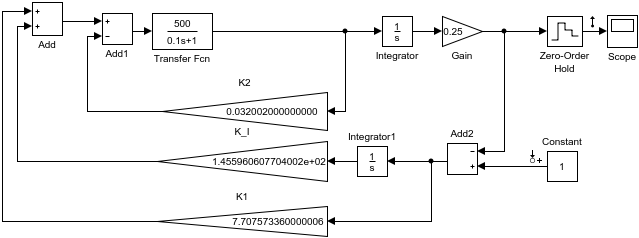
\includegraphics[width = 0.9\textwidth]{finModel}
		\caption{Схема моделирования системы с  ПИ регулятором}
		\label{finModel}
	\end{figure}
	
	\begin{figure}[ht!]
		\centering
		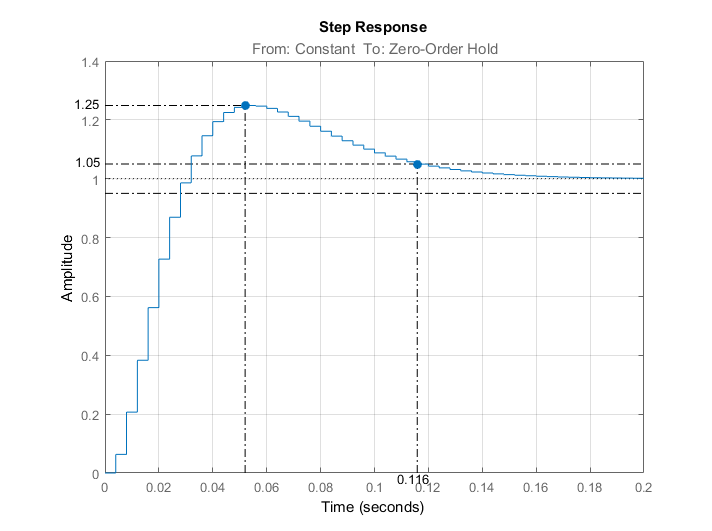
\includegraphics[scale=0.8]{fin}
		\caption{Переходный процесс системы с ПИ регулятором}
		\label{fin}
	\end{figure}
	\clearpage
	\section*{Вывод}
	Как указано на рисунке \ref{fin} время переходного процесса синтезированной системы $t_\text{пс} = 0,116c$, что удовлетворяет заданному условию $t_\text{п} = 0,15c$. Так же процент перерегулирования составил $\sigma = \displaystyle{\frac{1,25 - 1}{1}}\cdot100\% = 25\%$, что не превышает разрешённых 30\%. 
	
	Исходя из этого, синтез ПИ регулятора, удовлетворяющего заданным показателям качества системы, можно считать успешным.
	\clearpage
\section*{\begin{center} Приложение А\end{center}}

Листинг 1 --- программа нахождения значения матриц в дискретном пространстве
\begin{lstlisting}
	T = 0.004;
	An = [0, 0.25; 0, -10];
	Bn = [0; 5000];
	Ad = expm(A * T);
	Bd = 0;
	for i = 1:00
		Bd = Bd + (A^(i - 1) * T^(i))/(prod(1:i)) * Bn;
	end
\end{lstlisting}
\end{document}